\section{Manuale utente ed esecuzione}

\subsection{Avvio del Server}
Per consentire ai client di connettersi al server, è ovviamente necessario far partire il Server. Se si esege il codice da IntelliJ basta recarsi sul file \texttt{ChatServer.java} ed eseguirlo. L'output sarà il seguente: 
\begin{figure}[h]
  \centering
  \begin{minipage}{0.45\textwidth}
    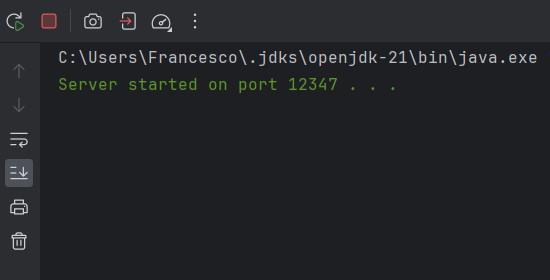
\includegraphics[width=\linewidth]{imagens/outputs/1.png}
    \caption{Avvio del Server}
  \end{minipage}\hfill
\end{figure}

\subsection{Avvio del Client}
Per iniziare a messaggiare con altri utenti connessi al server, è ovviamente necessario far una (o più) istanza del cliebt. Se si esege il codice da IntelliJ basta recarsi sul file \texttt{ChatClient.java} ed eseguirlo. In primo luogo, verrà richiesto il nome utente. L'output sarà il seguente: 
\begin{figure}[h]
  \centering
  \begin{minipage}{0.45\textwidth}
    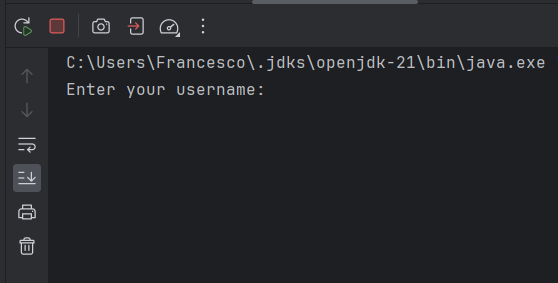
\includegraphics[width=\linewidth]{imagens/outputs/1_2.png}
    \caption{Avvio del client}
  \end{minipage}\hfill
\end{figure}
\newpage

\subsection{Accesso}
Per eseguire l'accesso al server, sarà sufficiente fornire l'username, che deve essere univoco. Nel caso in cui il nome inserito risulti già scelto da un'altro utente, verrà mostrato un messaggio di errore che invita l'utente ad inserirne uno differente.
\begin{figure}[h]
  \centering
  \begin{minipage}{0.45\textwidth}
    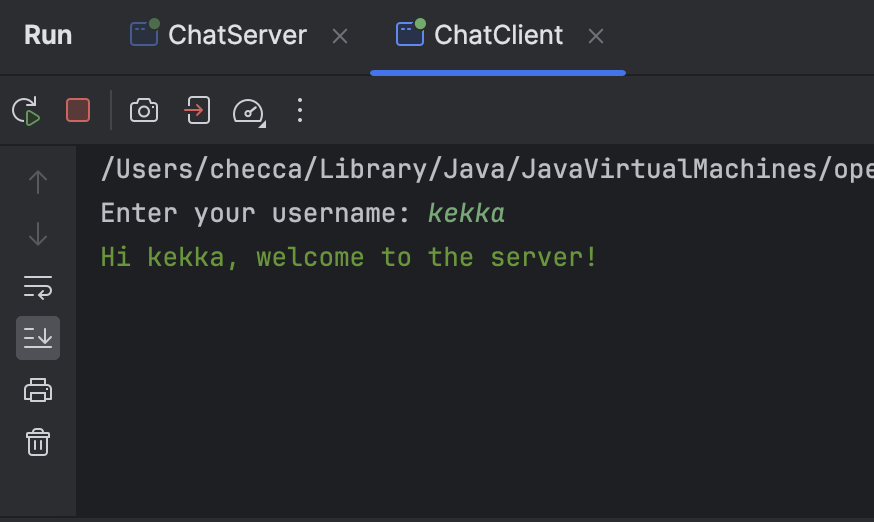
\includegraphics[width=\linewidth]{imagens/outputs/2.png}
    \caption{Inserimento nome utente valido}
  \end{minipage}\hfill
  \begin{minipage}{0.45\textwidth}
    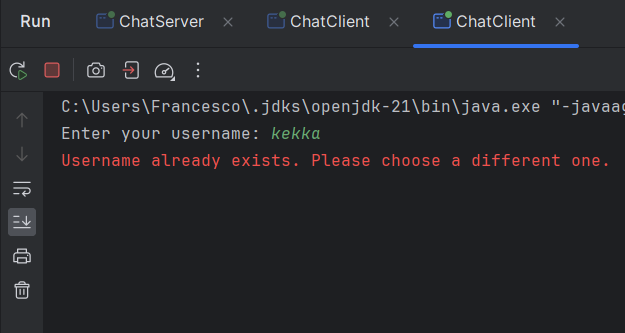
\includegraphics[width=\linewidth]{imagens/outputs/2_2.png}
    \caption{Inserimento nome utente già presente}
  \end{minipage}\hfill
\end{figure}
\newline
Come si può notare, è stato simulato l'inserimento da un'altro client di un nome utente già scelto e presente nel server.
\newline
Inoltre è stato previsto un sistema di LOG del server che monitora connessioni in entrata ed uscita. Di seguito è quindi riportata una rappresentazione grafica.
\begin{figure}[h]
  \centering
  \begin{minipage}{0.45\textwidth}
    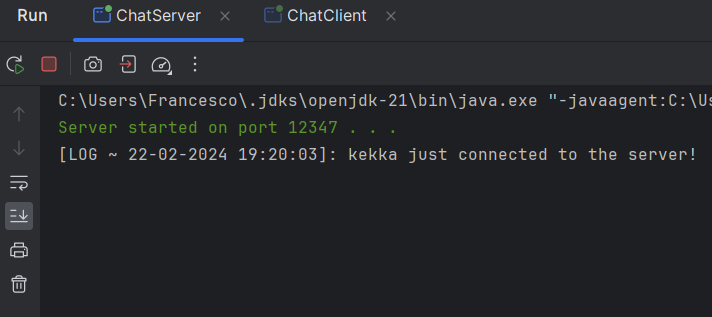
\includegraphics[width=\linewidth]{imagens/outputs/2_3.png}
    \caption{Visualizzazione log su Server}
  \end{minipage}\hfill
\end{figure}
\newpage

\subsection{Comandi di base}
\subsubsection{Join Channel}
\texttt{/join <canale>} è un comando che consente di entrare in un canale esistente. Il parametro \texttt{<canale>} rappresenta il nome del canale a cui desideri unirti. Ad esempio, \texttt{/join test} ti unirà al canale denominato "test". Nel caso in cui il canale non esista verrà mostrato un'errore.
\begin{figure}[h]
  \centering
  \begin{minipage}{0.45\textwidth}
    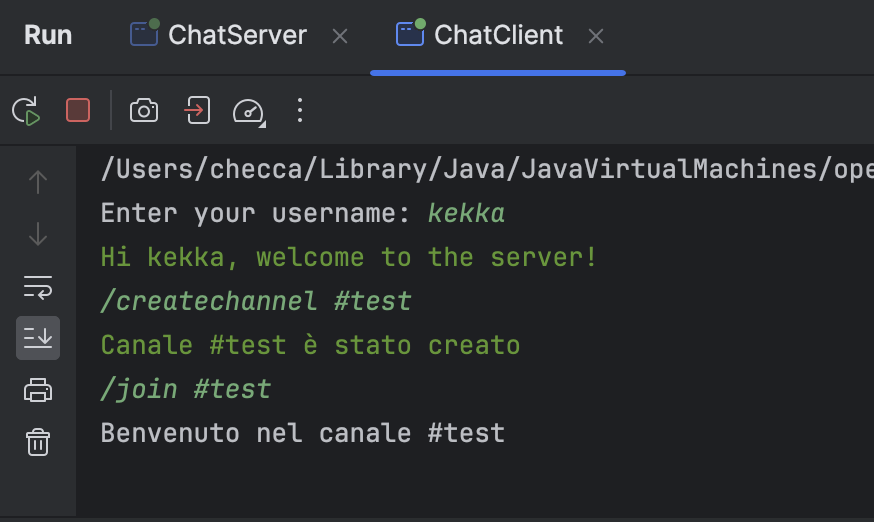
\includegraphics[width=\linewidth]{imagens/outputs/3.png}
    \caption{Creazione ed unione ad un canale}
  \end{minipage}\hfill
  \begin{minipage}{0.45\textwidth}
    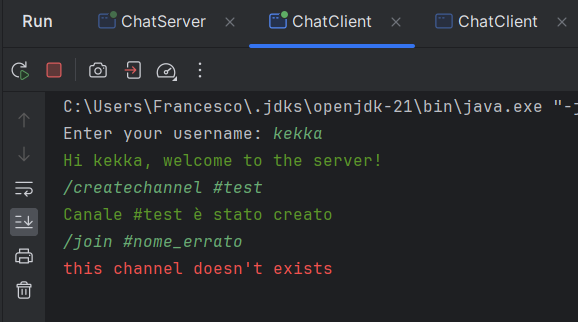
\includegraphics[width=\linewidth]{imagens/outputs/3_2.png}
    \caption{unione ad un canale inesistente}
  \end{minipage}\hfill
\end{figure}

\subsubsection{Leave Channel}
\texttt{/leave} è un comando utilizzato per abbandonare il canale corrente. Non richiede parametri aggiuntivi. Se eseguito in un canale notificherà a tutti gli utenti l'uscita dal canale e quindi permetterà l'uscita all'utente che lo ha eseguito. Altrimenti verrà mostrato un errore in quanto questo comando è esseguibile solo se si è in un canale.
\begin{figure}[h]
  \centering
  \begin{minipage}{0.45\textwidth}
    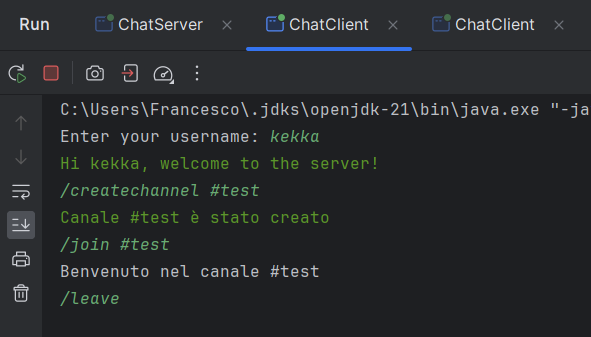
\includegraphics[width=\linewidth]{imagens/outputs/4.png}
    \caption{uscita da un canale}
  \end{minipage}\hfill
  \begin{minipage}{0.45\textwidth}
    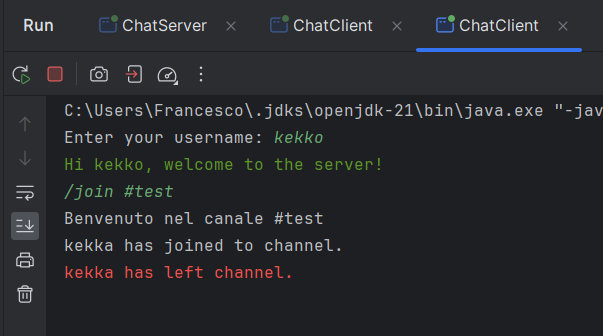
\includegraphics[width=\linewidth]{imagens/outputs/4_2.png}
    \caption{messaggio per i partecipanti}
  \end{minipage}\hfill
\end{figure}
\newpage

\subsubsection{Send Private Message}
\texttt{/privmsg <nickname> <messaggio>} è un comando che consente di inviare un messaggio in privato a un altro utente. Il parametro \texttt{<nickname>} rappresenta il nickname dell'utente a cui si vuole inviare il messaggio, mentre \texttt{<messaggio>} è il contenuto del messaggio che si desidera inviare. Nel caso in cui viene digitato il nome di un utente che non esiste (o che comunque non è connesso al server), verrà mostrato un'errore.
\begin{figure}[h]
  \centering
  \begin{minipage}{0.45\textwidth}
    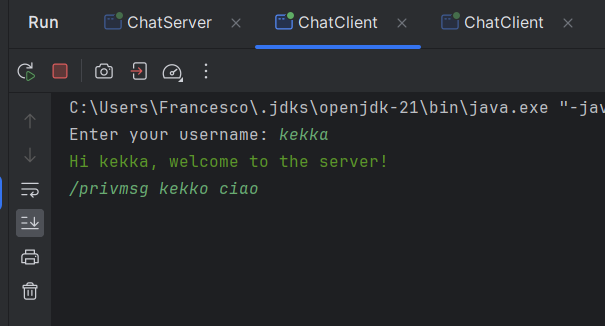
\includegraphics[width=\linewidth]{imagens/outputs/5.png}
    \caption{Invio messaggio in privato}
  \end{minipage}\hfill
  \begin{minipage}{0.45\textwidth}
    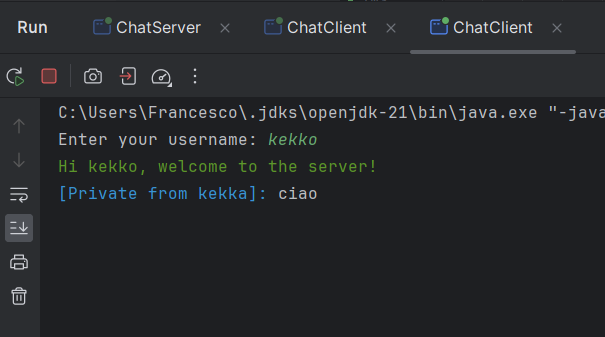
\includegraphics[width=\linewidth]{imagens/outputs/5_2.png}
    \caption{ricezione messaggio in privato}
  \end{minipage}\hfill
\end{figure}

\subsubsection{Send Message}
\texttt{/msg <messaggio>} è un comando che consente di inviare un messaggio nel canale corrente. Il parametro \texttt{<messaggio>} rappresenta il contenuto del messaggio che desideri inviare. Il messaggio sarà visibile a tutti gli utenti presenti nel canale in cui viene eseguito. Se eseguito quando non si è in un canale verrà mostrato un'errore in quanto questo comando è eseguibile solo se si è in un canale.
\begin{figure}[h]
  \centering
  \begin{minipage}{0.45\textwidth}
    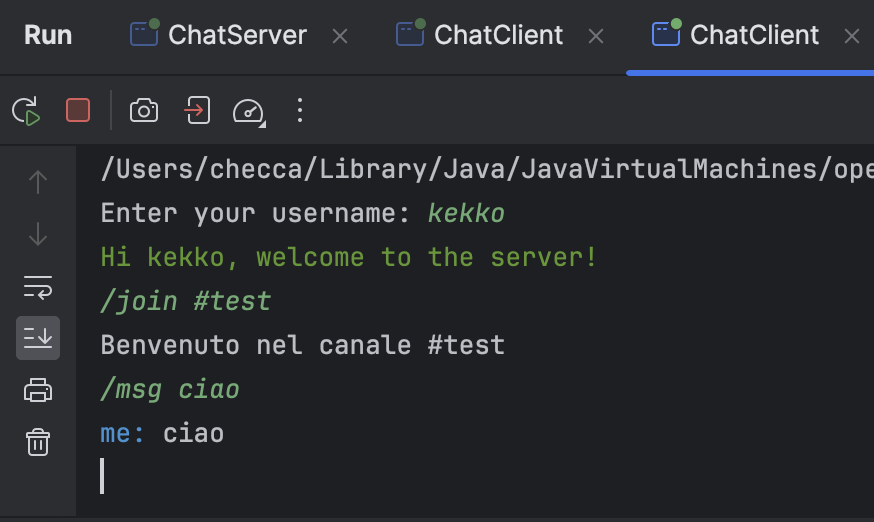
\includegraphics[width=\linewidth]{imagens/outputs/6.png}
    \caption{invio messaggio in un canale}
  \end{minipage}\hfill
  \begin{minipage}{0.45\textwidth}
    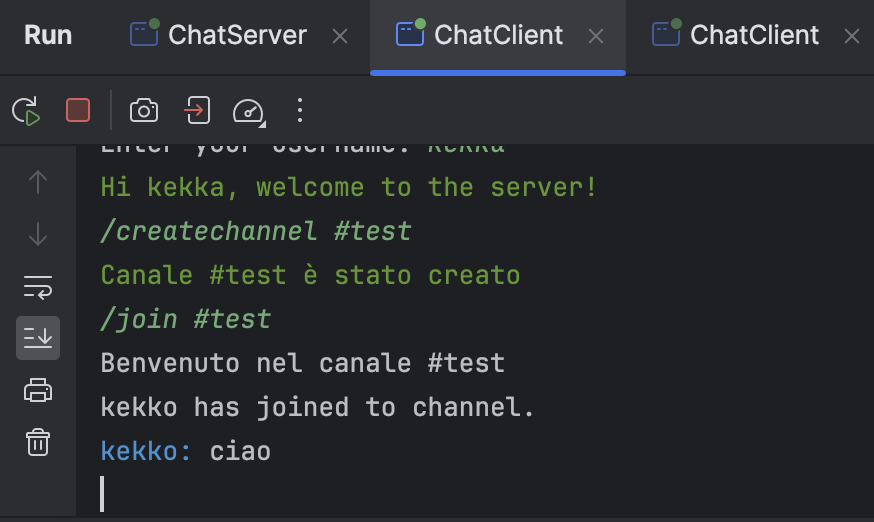
\includegraphics[width=\linewidth]{imagens/outputs/6_2.png}
    \caption{ricezione messaggio inviato in un canale}
  \end{minipage}\hfill
\end{figure}
\newpage

\subsubsection{List Users}
\texttt{/users} è un comando utilizzato per visualizzare un elenco degli utenti attualmente connessi al canale. Se eseguito quando non si è in un canale verrà mostrato un'errore in quanto questo comando è eseguibile solo se si è in un canale.
\begin{figure}[h]
  \centering
  \begin{minipage}{0.45\textwidth}
    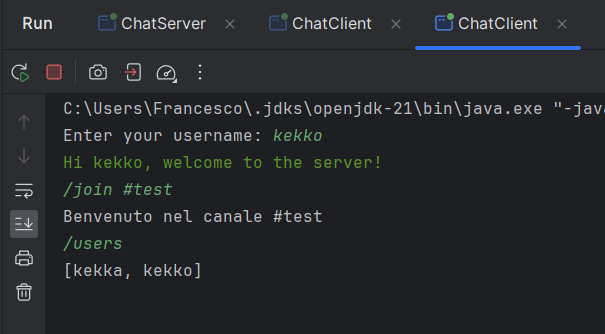
\includegraphics[width=\linewidth]{imagens/outputs/8.png}
    \caption{esecuzione comando in un canale}
  \end{minipage}\hfill
  \begin{minipage}{0.45\textwidth}
    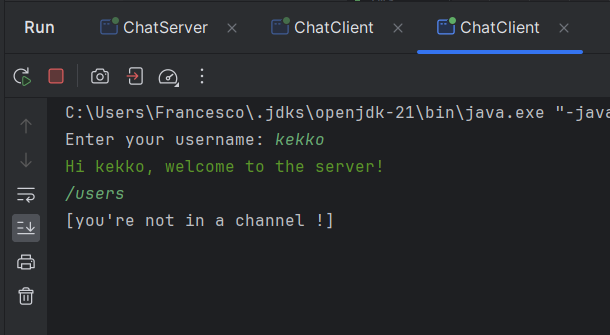
\includegraphics[width=\linewidth]{imagens/outputs/8_2.png}
    \caption{esecuzione comando NON in un canale}
  \end{minipage}\hfill
\end{figure}

\subsubsection{List Channels}
\texttt{/list} è un comando utilizzato per visualizzare un elenco dei canali attivi sul server. Può essere eseguito in qualunque momento.
\begin{figure}[h]
  \centering
  \begin{minipage}{0.45\textwidth}
    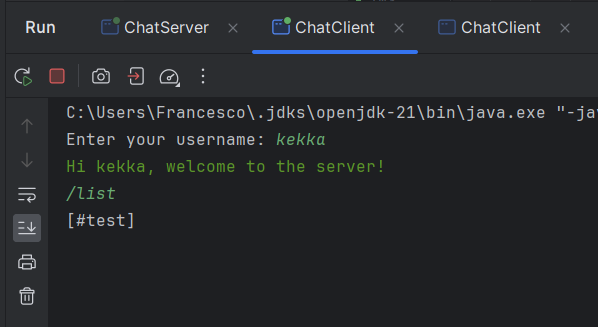
\includegraphics[width=\linewidth]{imagens/outputs/7.png}
    \caption{comando per mostrare i canali attivi}
  \end{minipage}\hfill
\end{figure}
\newpage

\subsection{Comandi admin}
\subsubsection{Kick User}
\item \texttt{/kick <nickname>} è un comando utilizzato dagli amministratori per espellere un utente dal canale. Il parametro \texttt{<nickname>} rappresenta il nickname dell'utente che si desidera espellere. Se il nome dell'utente inserito non esiste (o se comunque non è presente in quel canale) verrà generato un'errore. Inoltre, se eseguito quando non si è in un canale verrà mostrato un'errore in quanto questo comando è eseguibile solo se si è in un canale.
\begin{figure}[h]
  \centering
  \begin{minipage}{0.45\textwidth}
    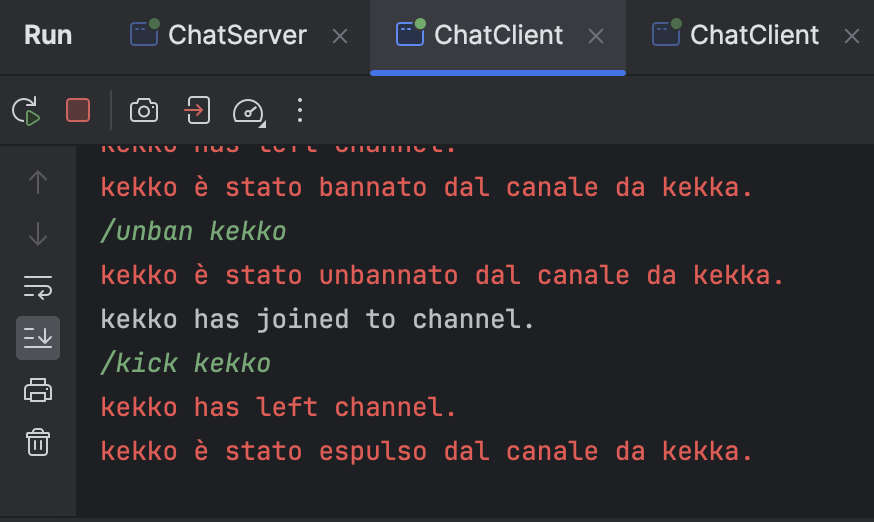
\includegraphics[width=\linewidth]{imagens/outputs/9.png}
    \caption{espulsione di un'utente}
  \end{minipage}\hfill
  \begin{minipage}{0.45\textwidth}
    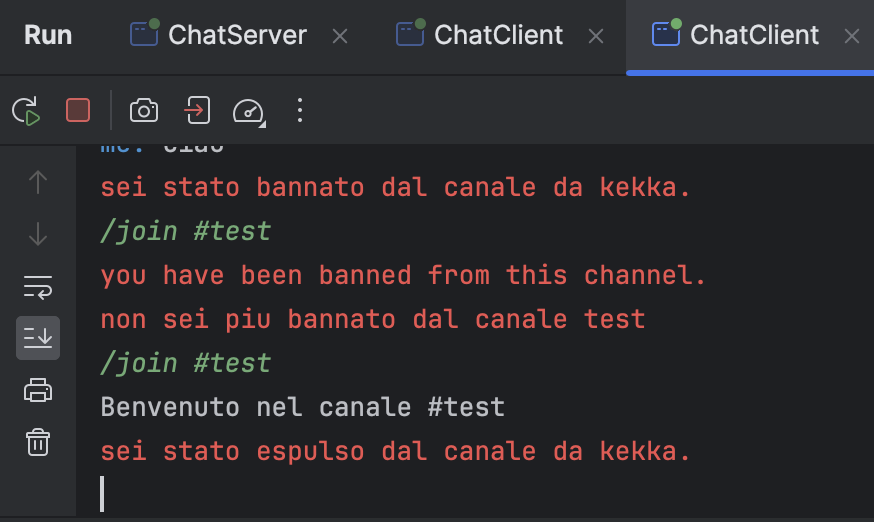
\includegraphics[width=\linewidth]{imagens/outputs/9_2.png}
    \caption{messaggio mostrato all'utente espulso}
  \end{minipage}\hfill
\end{figure}

\subsubsection{Ban User}
\item \texttt{/ban} è un comando utilizzato dagli amministratori per bannare un utente dal canale. Se il nome dell'utente inserito non esiste (o se comunque non è presente in quel canale) verrà generato un'errore. Inoltre, se eseguito quando non si è in un canale verrà mostrato un'errore in quanto questo comando è eseguibile solo se si è in un canale. Anche nel caso in cui l'utente da bannare risulta già bannato, verrà mostrato un'errore.
\begin{figure}[h]
  \centering
  \begin{minipage}{0.45\textwidth}
    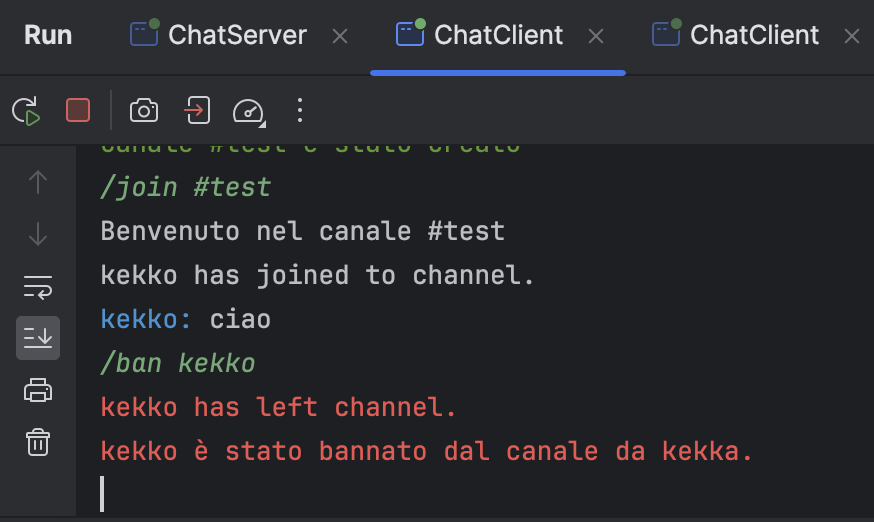
\includegraphics[width=\linewidth]{imagens/outputs/10.png}
    \caption{ban di un utente}
  \end{minipage}\hfill
  \begin{minipage}{0.45\textwidth}
    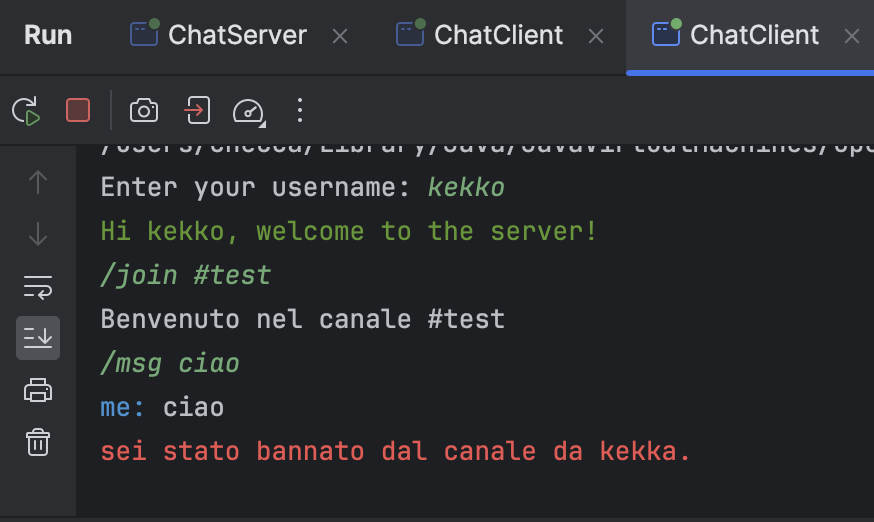
\includegraphics[width=\linewidth]{imagens/outputs/10_2.png}
    \caption{messaggio utnte bannato}
  \end{minipage}\hfill
\end{figure}
\newpage

\subsubsection{Unban User}
\item \texttt{/unban} è un comando utilizzato dagli amministratori per rimuovere un ban precedentemente impostato su un utente nel canale. Se il nome dell'utente inserito non esiste (o se comunque non è presente in quel canale) verrà generato un'errore. Inoltre, se eseguito quando non si è in un canale verrà mostrato un'errore in quanto questo comando è eseguibile solo se si è in un canale. Anche nel caso in cui l'utente dalla quale si vuole revocare il ban risulta non precedentemente bannato, verrà mostrato un'errore.
\begin{figure}[h]
  \centering
  \begin{minipage}{0.45\textwidth}
    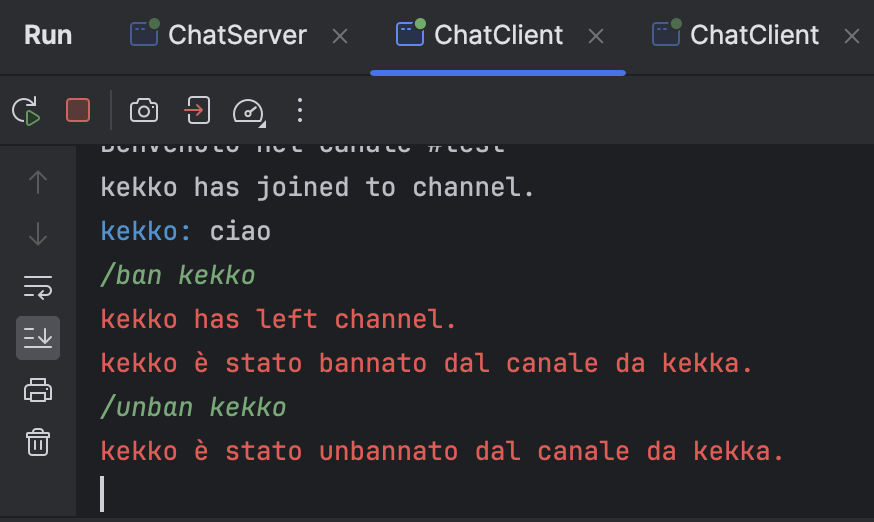
\includegraphics[width=\linewidth]{imagens/outputs/11.png}
    \caption{revoca ban utente}
  \end{minipage}\hfill
  \begin{minipage}{0.45\textwidth}
    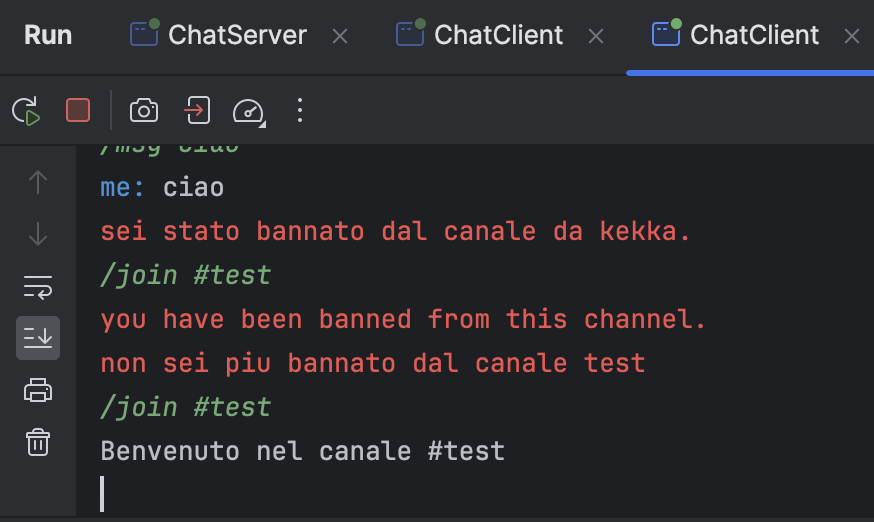
\includegraphics[width=\linewidth]{imagens/outputs/11_2.png}
    \caption{messaggio revoca ban utente}
  \end{minipage}\hfill
\end{figure}
\newline
Importante notare come, nella Figura \ref{fig:11_2}, l'utente precedentemente bannato, abbia cercato di accedere al canale a cui era appena stato bannato. Gli viene mostrato un'errore poichè non gli è consentito l'accesso in quanto bannato. Solamente dopo la revoca del ban all'utrente gli sarà concesso nuovamente l'accesso a quel canale.

\subsubsection{Promote User}
\item \texttt{/promote <nickname>} è un comando utilizzato dagli amministratori per promuovere un utente a un ruolo con privilegi aggiuntivi nel canale. Se il nome dell'utente inserito non esiste (o se comunque non è presente in quel canale) verrà generato un'errore. Inoltre, se eseguito quando non si è in un canale verrà mostrato un'errore in quanto questo comando è eseguibile solo se si è in un canale.
\begin{figure}[h]
  \centering
  \begin{minipage}{0.45\textwidth}
    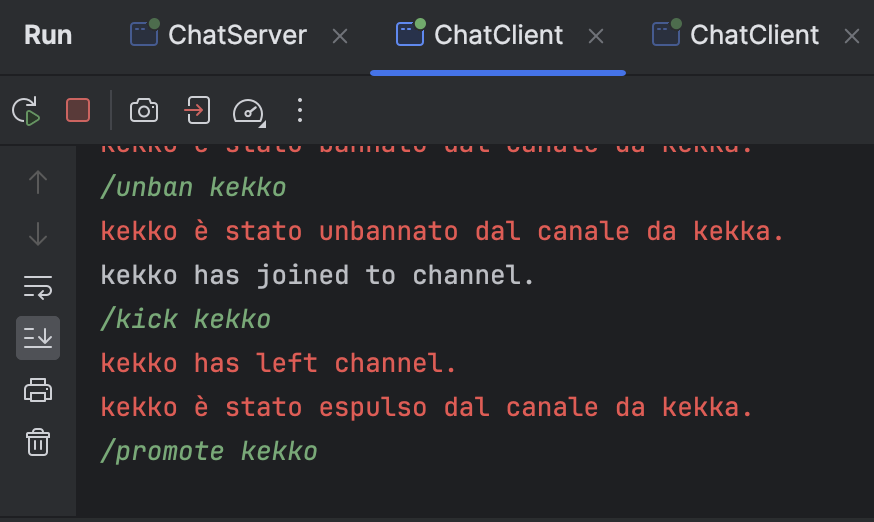
\includegraphics[width=\linewidth]{imagens/outputs/12.png}
    \caption{promozione di un utente}
  \end{minipage}\hfill
  \begin{minipage}{0.45\textwidth}
    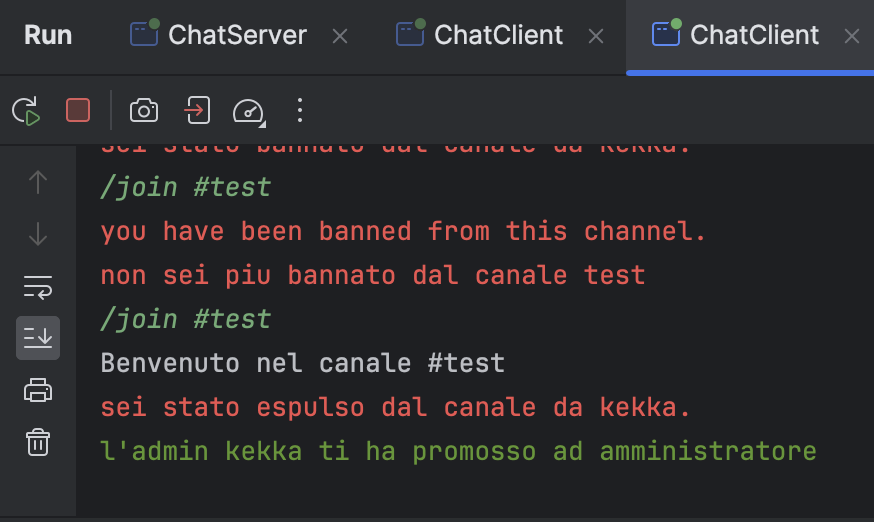
\includegraphics[width=\linewidth]{imagens/outputs/12_2.png}
    \caption{messaggio di avviso all'utente appena promosso}
  \end{minipage}\hfill
\end{figure}

\textbf{N.B.}: \textit{Solamente per brevità, non sosno stati mostrati tutte le possibile combinazioni di errori.}